\documentclass[tikz]{standalone}
\usepackage[outline]{contour}

\begin{document}
	    \contourlength{1.5pt}
	    	    \contourlength{1.2pt}
	    
	    \tikzset{
	    	double arrow/.style args={#1 colored by #2 and #3}{
	    		-stealth,line width=#1,#2, % first arrow
	    		postaction={draw,-stealth,#3,line width=(#1)/3,
	    			shorten <=(#1)/3,shorten >=2*(#1)/3}, % second arrow
	    	}
	    }
\begin{tikzpicture}
    \node[anchor=south west,inner sep=0] at (0,0) {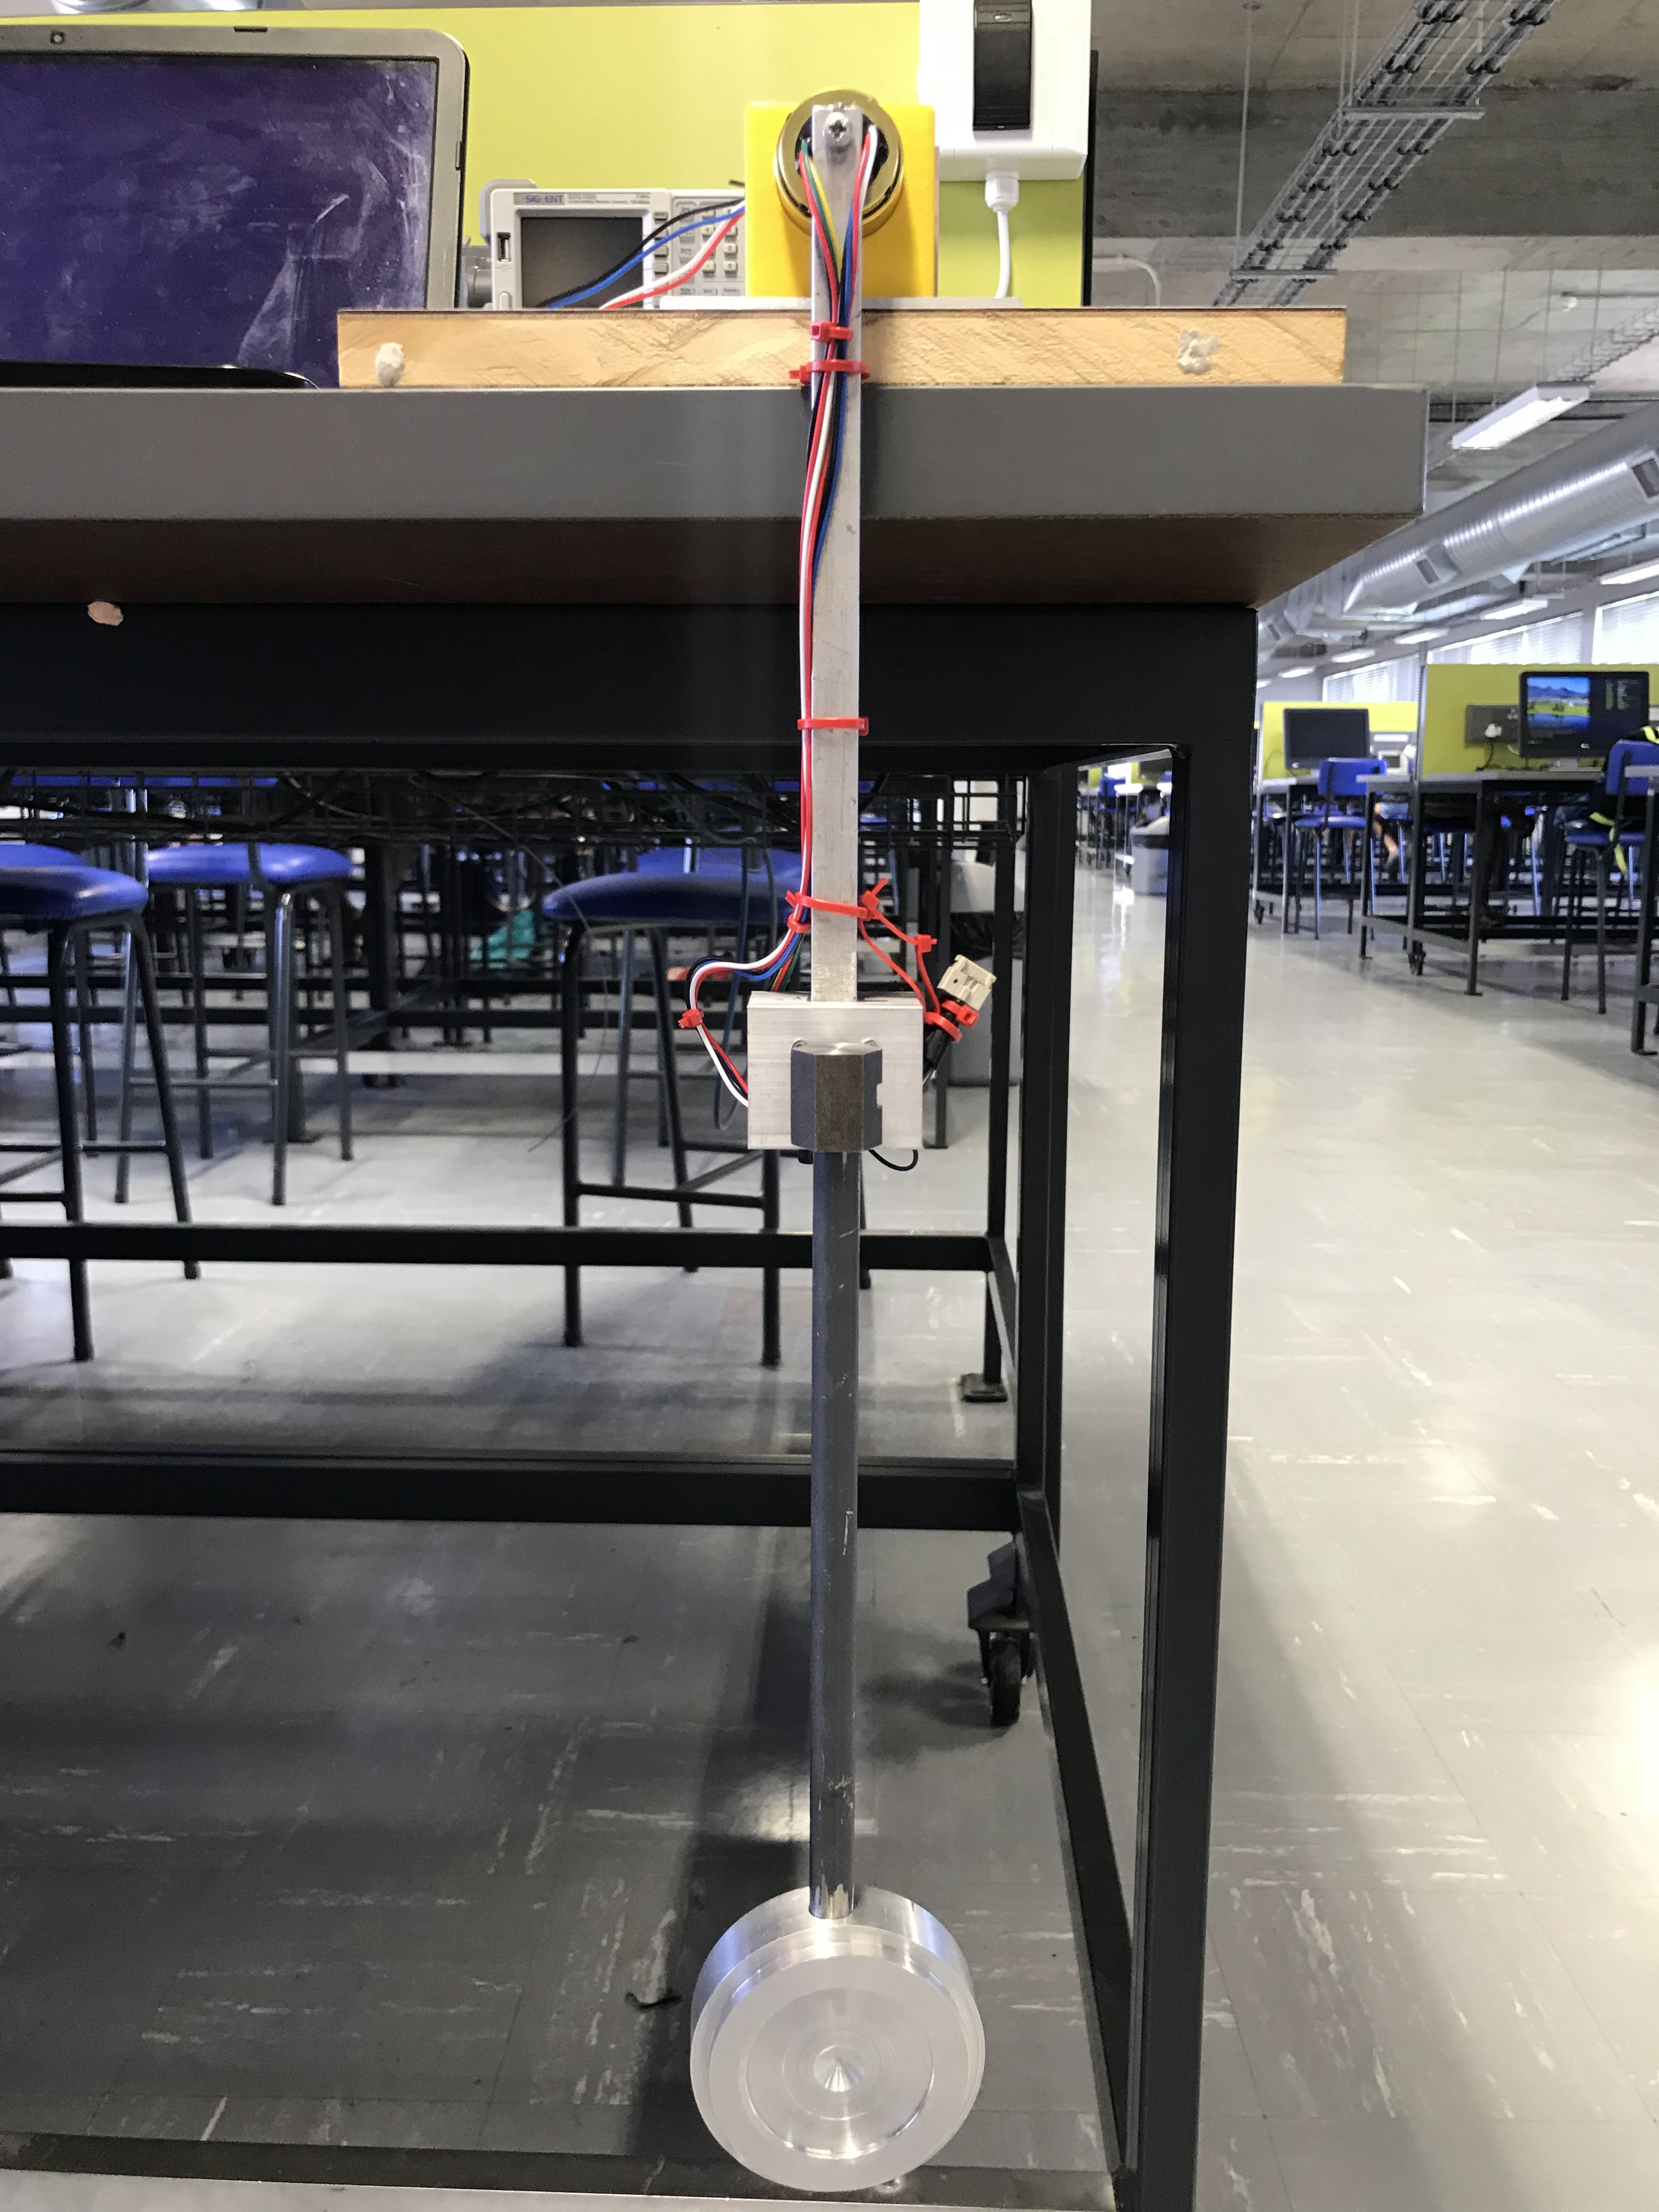
\includegraphics[width=\textwidth]{overview.jpg}};
    %microcontroller
    %\draw[green,ultra thick,rounded corners] (6.5,5) node[above]{ \textbf{MCU} };
    

    
    
    
    \draw[double arrow=2pt colored by black and white] (6,5) -- (8,5) node[right,white]{\contour{black}{\textbf{Actuated Pendulum}}};
    
    \draw[double arrow=2pt colored by black and white] (6,12) -- (8,12) node[right,white]{\contour{black}{\textbf{Unactuated Pendulum}}};
    
    \draw[double arrow=2pt colored by black and white] (6,8) -- (8,8) node[right,white]{\contour{black}{\textbf{Torque Input \& Hinge}}};	
    
    \draw[double arrow=2pt colored by black and white] (6.2,15) -- (8,15) node[right,white]{\contour{black}{\textbf{Fixed Hinge}}};	
    %XOR
    
    
\end{tikzpicture}
\end{document}